\documentclass[]{article}

\usepackage[style=ieee,backend=bibtex]{biblatex}
\PassOptionsToPackage{margin=1in}{geometry}
\usepackage{wordlike}
\usepackage{setspace}
\usepackage{parskip}
\usepackage{graphicx}

\setstretch{1.5}


%opening
\title{How Open is Open Source? Metrics for measuring software mutation}
\author{Charles Hathaway}

\bibliography{biblo}

\begin{document}

\maketitle

\begin{abstract}

Open source software is toted as being "openly accessible" to many people, thus allowing greater innovation and complex new methodologies.
However, given the complexity of software and how difficult it is to design and implement, the question of whether or not secondary communities adapt and modify the software needs to be addressed.
This paper poses the question of determining the involvement of multiple communities to a project by measuring their contributions in terms of complexity, and discusses how we would go about measuring contributions to a project in a meaningful way.

\end{abstract}

\section{Introduction}

% What is open source? very brief regurgitation
% Why do we care about open source? list large projects that "matter"
% --> Include projects listed as "can not fail" internet services
% Does it matter how open projects are?
% How will being able to measure how open projects are help organize things

Open Source software, which includes such well known projects as Linux, Apache, and OpenSSL, has a large portion of todays market share in their respective segments.
According to reports available from w3techs \cite{w3techs2015usage}, *nix systems account for 67.7\% of the internet web servers; 52.7\% of these are running a Linux distribution. 
Important projects, such as OpenSSL, attract world-wide media attention when sever bugs appear; take for example the numerous articles published because of the April 2014 bug called "Heartbleed" \cite{mitre2013heartbleed}  \cite{whittaker2014heartbleed}.

After this particular crisis, it was realized that there are numerous open source projects that are too big to fail.
Large corporations agreed to contribute money to these projects, in hopes that it will prevent another such bug \cite{brodkin2014heartbleed}.
It is here where we can begin to understand the need to figure out who is working on projects, how much are they doing, and how complicated the projects are.

Understanding who is working on a project is no simple matter; we must consider multiple roles (programmer, tester, project manager, to name a few), along with the amount of work they are putting into that project (are they spending 1/8 of their day on it? 16/24 of their day?).
In this paper, will propose a method for further research that will allow one to quantify the contributions of at least one role in a software developers world; the role of the programmer.
Namely, what we want to discover is how we can measure the change that a developer causes in the codebase; are they simply renaming variables, adding UI elements, or changing core algorithms?

This forays into the field of software complexity.
Do not confuse this field with other forms of complexity we often look at in the computer science discipline, such as time and space complexity.
The goal of this field is to determine how difficult a program is to understand, test, and write.
We will not be focusing on developing another metric to just determine how complex a program is; rather, we will concern ourselves the change of complexity as function of time (where time can be commits, space-time, or something as arbitrary as lines of code).

There have been many attempts over the years to measure software complexity; some of the most well known ones by McCabe \cite{ref:a_complexity_measure}, Oviedo \cite{ref:oviedo1993control}, and Halstead \cite{ref:halstead1977elements}.
Our goal in this paper is to evaluate the most common complexity measures, and look for correlations between how real people percieve a program to be, and how the metrics understand the complexity of a program.
To conclude the paper, we will run a small-scale experiment on 5 people, asking them to rank 5 projects (which produce similar output) on how complex they appear to be.
Later research would repeat this experiment on a larger, and more diverse, group of subjects.

For simplicity, this paper will utilize the visual programming environment created for the 3Helix program at Rensselaer Polytechnic Institute, CSnap.
These scripts are best stored (for long term access) as images, and will be included at the end of the paper.

\section{Literature Review}

% We have at least 2 distinct "areas" to review; open source-ness, and ways of measuring software similiarity

As a form of literature review, will use a subset of well-known papers that represent some of the most important works in this field.
Most of these articles have been reprinted \textbf{Software Engineering Metrics Volume 1} \cite{sheppherd1993complexity}, including:
\begin{itemize}
	\item \textbf{A Complexuty Measure} \cite{ref:a_complexity_measure}
	\item \textbf{Control Flow, Data Flow, and Program Complexity} \cite{ref:oviedo1993control}
\end{itemize}

It is worth mentioning that most of these metrics have had their accuracy questioned, and for the most part been proven to fail in one or more ways.
A very well known paper that described the failure of these metrics is \textbf{Evaluating Software Complexity Measures}, written in 1988 by Elaine J. Weyuker \cite{ref:evaluating_software_complexity_measures}.
The analysis done in this paper has been used as the core for many following software complexity papers, including the recent publication by Hongwei Tao, \textbf{Complexity measure based on program slicing and its validation} \cite{ref:tao2014complexity}.


% More stuff?

\subsection{Evaluating Software Complexity Measures}

% We need to talk about everything, including silly things like...
% Lines of code changed

In this section, we will summarize and describe previous metrics considered.
Weyuker wrote a paper in 1988\cite{ref:evaluating_software_complexity_measures} which considered many of these metrics, and we will therefore make references to her paper.
For convenience, I have copied the 9 properties of complexity measures she proposed here. 
Note, however, that they are explained in greater detail in the paper.

\begin{itemize}
	\item Property 1: $(\exists P)(\exists Q)(|P|\neq |Q|)$
	\item Property 2: Let c be a nonnegative number. Then there
are only finitely many programs of complexity c.
	\item Property 3: There are distinct programs P and Q such
that $|P| ~= ~|Q|$
	\item Property 4: $(\exists P)(\exists Q)(P \equiv Q ~\& ~|P| \neq |Q|)$
	\item Property 5: $(\forall P)(\forall Q)(|P| \leq |P; Q| ~and ~|Q| \leq |P; Q|)$
	\item Property 6a: $(\exists P)(\exists Q)(\exists R)(|P| = |Q| \& |P;R| \neq |Q; R|)$
	\item Property 6b: $(\exists P)(\exists Q)(\exists R)(|P| = |Q| \& |R;P| \neq |R; Q|)$
	\item Property 7: There are program bodies P and Q such that Q is formed by permuting the order of the statements of P, and $|P| \neq |Q|$
	\item Property 8: If P is a renaming of Q, then $|P| = |Q|$
	\item Property 9: $(\exists P)(\exists Q)(|P|+|Q| < |P; Q|)$
\end{itemize}

\subsection{Cyclomatic complexity}

Thomas McCabe proposed a complexity measure in his 1976 paper \cite{ref:a_complexity_measure}.
In this section, I will briefly describe how it works, how to calculate it, and discuss some responses to it (specifically the responses made by  Elaine Weyuker in her 1988 paper \cite{ref:evaluating_software_complexity_measures}).

\subsubsection{How it works}

The McCabe metric (Cyclomatic number) analyses the control flow of a program to determine how complex it is. 
There are 3 primary items that is used the calculation of the cyclomatic number:
\begin{itemize}
	\item Number of nodes, denoted as n
	\item Number of edges, denoted as e
	\item Number of compontents, denoted as p
\end{itemize}

Given these three variables, we can calculate a complexity (v) of a program using the following equation:

$v ~= ~e ~- ~n ~+ 2p$

The real challenge is to create the graph so you can find values for these variables.
To do this you must break a program into parts such that there is a starting node, and ending node, and a sequence of nodes between that two have the following key attributes:
\begin{itemize}
	\item A compound statement is only one node; ie, int i=0; i = b*x; ... counts as only one node until the next branch occurs
	\item A branch is a conditional, either in the form of an if statement or a loop (with a loop, connect the node to both the following statement(s) and the code that gets executed after it exits)
\end{itemize}

As a general rule of a thumb, we have a component anywhere a loop occurs.
We can have multiple components inside a component (embedded loops). 

Once we have created a graph, it is a trivial matter of counting the number of edges, nodes, and components and applying the equation.

\subsubsection{Analysis}

This metric was included in the analysis performed by Weyuker in her 1988 paper \cite{ref:evaluating_software_complexity_measures}.
Ultimately, she concluded that McCabes metric failed to address properties 2, 6, 7, and 9.
Additional critique was made by Martin J. Shepperd in his 1988 paper \cite{shepperd1988critique}, however we found some discrepancies between this critique and the model developed by McCabe.

\subsection{Normalized Compression Distance}

Proposed by Rudi Cilibrasi and Paul Vitanyi in their 2005 paper, \textbf{Clustering by compression} \cite{ref:cilibrasi2005clustering} puts forth a very straightforward way of calculating complexity changes between two pieces of code, without even knowledge of the structure of the content.
They proposed using a standard compression method (such as gzip or PPMZ) to approximate the Kolmogorov complexity of a program, and using this solve the equation in figure \ref{ncd_eq_1}.


\begin{figure}[h]
	\caption{Normalized Compression Distance}
	\label{ncd_eq_1}
	\centering
	$NCD(x,y) ~= \frac{C(xy) - min(C(x),C(y))}{max(C(x),C(y))}$
\end{figure}

%\subsection{Effort measure}
% Forgo this section for now, I'm missing the book where it is defined
% Need to trace this back I think
% This is sort of the thing that Ron's expirement would look at
%\cite{ref:evaluating_software_complexity_measures}

\subsection{Data flow complexity}

Enrique Oviedo proposed a metric based on data flow in his 1980 paper \cite{ref:oviedo1993control}.
This metric is based on 2 key components; data flow (DF) and control flow (CF).
He concludes with the equation $C = \alpha CF + \beta DF$ (where $\alpha=\beta=1$).
% This later followed up be ... who said \alpha should equal and \beta should equal...

\subsubsection{How it works}

Control flow is simply the cardinality of the program flow graph.
The program flow graph, and how to construct it, is clearly defined in the paper.
It more or less follows the same structure as the graphs we construct for the Cyclomatic number, with a more formal definition being given to how a "program" (function in modern terminology) is denoted.
Formally,

$CF=\parallel E\parallel$

Where $\parallel ~\parallel$ stands for set cardinality.

The more complicated part of this metric is the data flow measure.
The key terminology for this measure is the distinction between a locally available variable and a locally exposed variable.
A variable is locally available when the variable is defined in the block (a block is a "node" in our control flow).
A variable is locally exposed when it is referenced without being defined in the block.
Another important note is that a variable can be "overridden" in a block if it is locally exposed, and then made locally available. 

$DF_i = \sum\limits_{j=1}^{\parallel V_i \parallel} DEF(v_j)$

Where $V_i$ is the set of exposed variables in this block and $DEF(v_j)$ counts the number of available definitions for $v_j$.

$DF = \sum\limits_{i=1}^{\parallel S \parallel} DF_i+DF_f$

Where S is all nodes except the start and the end nodes.

\subsubsection{Analysis}

This metric was included in the analysis performed by Weyuker in her 1988 paper \cite{ref:evaluating_software_complexity_measures}.
Ultimately, she concluded that the Dataflow metric failed to address properties 2 and 5.

\subsection{Other metrics}

In addition to the above stated metrics, we will also consider lines of code (also referred to as statement count).
This metric is almost universally accepted as not indicative of the complexity of a program, and will provide a sane reference point to verify that we are not just finding correct data.

Lines of code is very dependent on the language in which we are evaluating programs.
Since we are using CSnap as a small-scale staging run, we will consider a "line of code" to be a command block (as defined by Snap! and CSnap).
These blocks include things such as "if", "go to {x coordinate}", etc.

\section{Measuring change}

% We really need to decide what to do about this :(

% Propose new metric in this paper and test with the toy example (small)

% Most likely an aggregate metric, but what weights and metrics?

There are several issues that need to be addressed by our algorithm of we are to effectively measure change in software over a large period of time.
These include:
\begin{itemize}
	\item Accounting for "non-changes"; ie, making a change to a project, testing it, then changing it back
	\item Discerning between changes that required little to no effort, and changes that may only have been to a line or two, but required a great deal of effort
	\item Considering things that change the output as part of the metric; not all changes will change the end-result of a program, but will rather optimize the process; other changes will cause the behavior of the program to dramatically alter. How do we differentiate these things?
\end{itemize}

\section{Experiment proposals}

% Ron's proposal goes in here;
% As a remind for the me that forgets later;
% --> Design a base CSnap project
% --> Modify the project to target a specific metric
% ---> This will be done multiple times; 1 project for each metric, then combinations
% --> Ask "people" which projects represent the most change, the least
% --> See which metrics agree with the responses the most

In order to test our complexity measure, we will first apply it to the domain of education and student progress.
The first step of entering this domain is to interface with the primary stakeholders; teachers and educations that work in the schools, with the primary audience; students.
Rather than trying to "ask" opinions and talk in an abstract way, we have developed a system to measure the change in student work on our CSnap "community site", which teachers can use to help us find a relationship between the various metrics discussed and complexity as viewed by teachers.

Before getting input from teachers, a survey needs to be developed and tested.
It will consists of a small number of scripts, which have varying degrees complexity.
The teachers will ultimately look at these scripts, and provide an absolute and relative complexity ranking that we can use to help calibrate our metric to present them with a very solid example to base their more qualitative feedback on.
Before presenting to the teachers, we will test the survey on fellows in the GK12 grant to verify the correctness and understandability of the survey.
In the next section, our initial results will be documented.

\section{Pre-experiment Results}

For this first draft, we created a survey consisting of the following questions
\begin{enumerate}
	\item Please rank the above projects from most complex (5) to least complex (1)
	\begin{itemize}
		\item Alpha
		\item Beta
		\item Bravo
		\item Charlie
		\item Delta
	\end{itemize}
	\item How complex would you rate each project (1 = not very complex, 100 = very complex)
	\item What is your gender?
	\begin{itemize}
		\item Female
		\item Male
	\end{itemize}
	\item Which race/ethnicity best describes you? (Please choose only one.)
	\begin{itemize}
		\item American Indian or Alaskan Native
		\item Asian / Pacific Islander
		\item Black or African American
		\item Hispanic American
		\item White / Caucasian
		\item Multiple ethnicity / Other (please specify)
	\end{itemize}
	\item What was your major?
\end{enumerate}

The scripts presented to the subjects can be seen in figures \ref{alpha}, \ref{beta}, \ref{bravo}, \ref{charlie}, and \ref{delta}

\begin{figure}[fh!]
	\caption{Calculate Metrics for Scripts}
	\label{calculate_metrics}
	\centering
	\begin{tabular}{l || c | c | c | c| c }
		& Cyclomatic & Dataflow & NCD & Lines of Code \\
		Alpha & -1 & 1 & 0.054 & 23 \\
		Beta & 2 & 6 & 0.031 & 14 \\
		Bravo & -1 & 1 & 0.039 & 11 \\
		Charlie & 6 & 28 & 0.056 & 25 \\
		Delta & 9 & 24 & 0.06 & 19
	\end{tabular}
\end{figure}

Figure \ref{calculate_metrics} shows the calculate metrics of each of the scripts.
These metrics were calculated via a program which will be included with the follow work to this paper, or when requested.
NCD in this table represents a comparison between the given project, and Alpha. 
We used Alpha as a based project, and calculated the NCD in relation to that project.
Interestingly, for 2 identical programs we ended with a wildly different NCD.

\begin{figure}[h]
	\caption{Sample Project Alpha}
	\label{alpha}
	\centering
	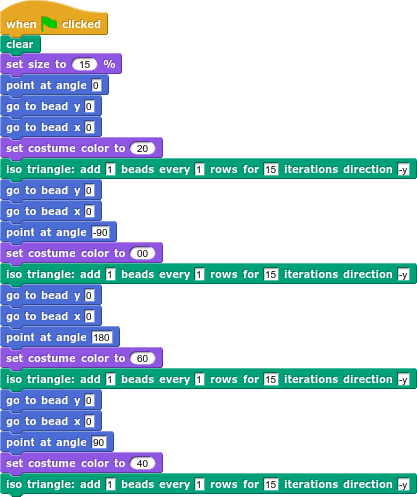
\includegraphics{sample_csnap_applications/alpha.png}
\end{figure}

\begin{figure}[h]
	\caption{Sample Project Beta}
	\label{beta}
	\centering
	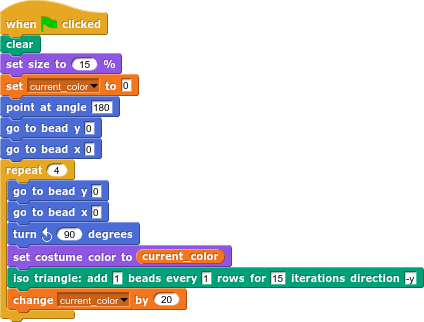
\includegraphics{sample_csnap_applications/beta.png}
\end{figure}

\begin{figure}[h]
	\caption{Sample Project Bravo}
	\label{bravo}
	\centering
	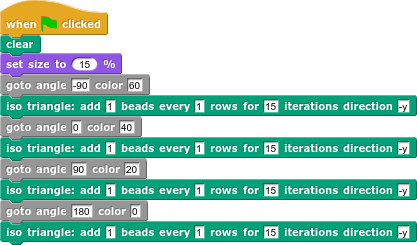
\includegraphics{sample_csnap_applications/bravo.png}
\end{figure}

\begin{figure}[h]
	\caption{Sample Project Charlie}
	\label{charlie}
	\centering
	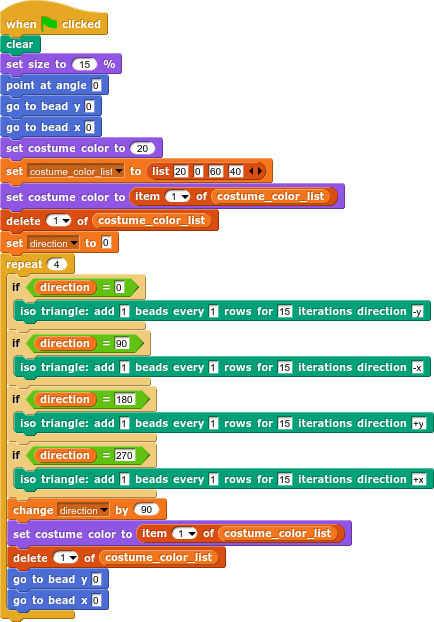
\includegraphics{sample_csnap_applications/charlie.png}
\end{figure}

\begin{figure}[h]
	\caption{Sample Project Delta}
	\label{delta}
	\centering
	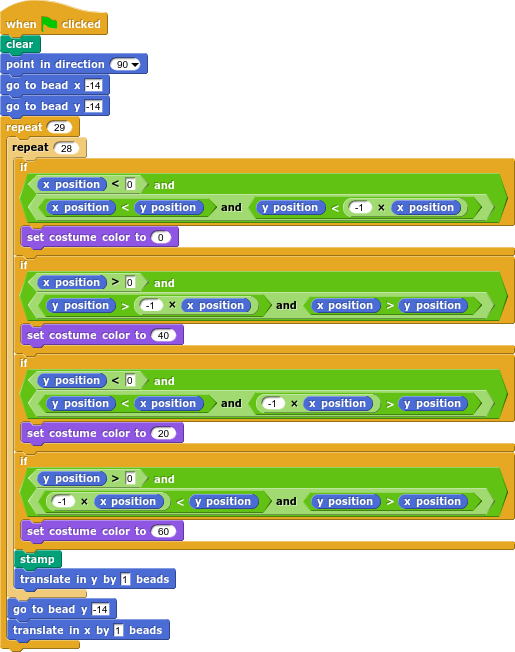
\includegraphics{sample_csnap_applications/delta.png}
\end{figure}

% Repeat with other groups; programmers, crowd sourcing

\section{Conclusion}
%% Moorthy
%% Please add papers in bibtex format
%%

\printbibliography

\end{document}
